\subsubsection{Model validation using utilization estimation} \label{sec-strategy-4-1}

The validation of the designed quantitative model was conducted based on a simplified model for which utilization is computed using theoretical calculations. The following conditions have been applied:
\begin{itemize}
	\item Starting rate of jobs is defined as a random variable with distribution denoted as SRD;
	\item Execution time of jobs is defined as a random variable with distribution denoted as ETD;
	\item Number of nodes used (requested) by examined jobs is defined as a random variable with distribution denoted as NND.
\end{itemize}

With this model it is possible to estimate the expected utilization achieved in a given long period of time. The expected utilization $U(t)$ depends on particular values of the random values in it, therefore it is mutable. But for big numbers of the time $t$ it is possible to take advantage of the law of large numbers (LLN). In this case, it can be argued that the value of $U(t)$ will tend to the same value, regardless of particular values of the random variables within it.

The theoretically calculated utilization for large values of $t$ can be estimated by the following equation:
\begin{equation}
	\label{eq-theoretical-utilization}
	U(t) \approx t \times E(SRD) \times E(ETD) \times E(NND)
\end{equation}
where $E(x)$ is the expected value (mathematical expectation) of a random variable. The next step was to compare the outcome of Equation~\ref{eq-quantitative-model} (model) and Equation~\ref{eq-theoretical-utilization} (theoretical estimation). Thereby, the expected value was calculated approximately, while going from the distribution function of a random variable to the utilization derivation.

Parameters of the experiment:
\begin{itemize}
	\item Starting rate is a random variable with the Poisson distribution, the event rate (i.e., rate parameter and considered as an expected value) $\lambda = 100$;
	\item Execution time is a random variable with the Normal distribution, mean of the distribution $\mu = 4$;
	\item Number of nodes used by a single job is a random variable with the Poisson distribution, $\lambda = 8$;
	\item Examined time interval is half a year $\approx4320\ hours$.
\end{itemize}

Results of the experiment: the utilization calculated using Equation~\ref{eq-quantitative-model} is equal to $13,822,864$, while the utilization calculated using Equation~\ref{eq-theoretical-utilization} (theoretical, based on expected values of SRD, ETD, NND only) is equal to $13,824,000$. Thus, the results are very close, and the little difference is due to approximations related to conducted computations.


\subsubsection{Model validation based on mathematical calculations and synthetic data from the simulator} \label{sec-strategy-4-2}

The further analysis of the quantitative model and the simulator is a simplified validation process that demonstrates equal results of both with the same input data.

The following common parameters are chosen: 
\begin{itemize}
    \item the total number of nodes is equal to 1;
    \item expected value ($\mu$) and variance ($\sigma^2$) for random parameters of job's waiting and execution times respectively are equal to 1; 
    \item the total processing time is equal to 5000 time units (hours).
\end{itemize}

Simulation process follows additional specific parameters:
\begin{itemize}
    \item job waiting time is defined according to the Poisson distribution;
    \item job execution time is defined according to the Normal distribution;
    \item job launching scheme: one stream and there is always one job in the queue;
    \item the total number of simulation runs is equal to 100.
\end{itemize}
Figure~\ref{fig-simulation-and-modeling} shows the plot with two lines that represent the probability that a given utilization will be achieved in a given time interval (that is defined by the total processing time): the blue line corresponds to the results obtained using the simulator, while the red line corresponds to calculations with the quantitative model.

\begin{figure}
    \centering
    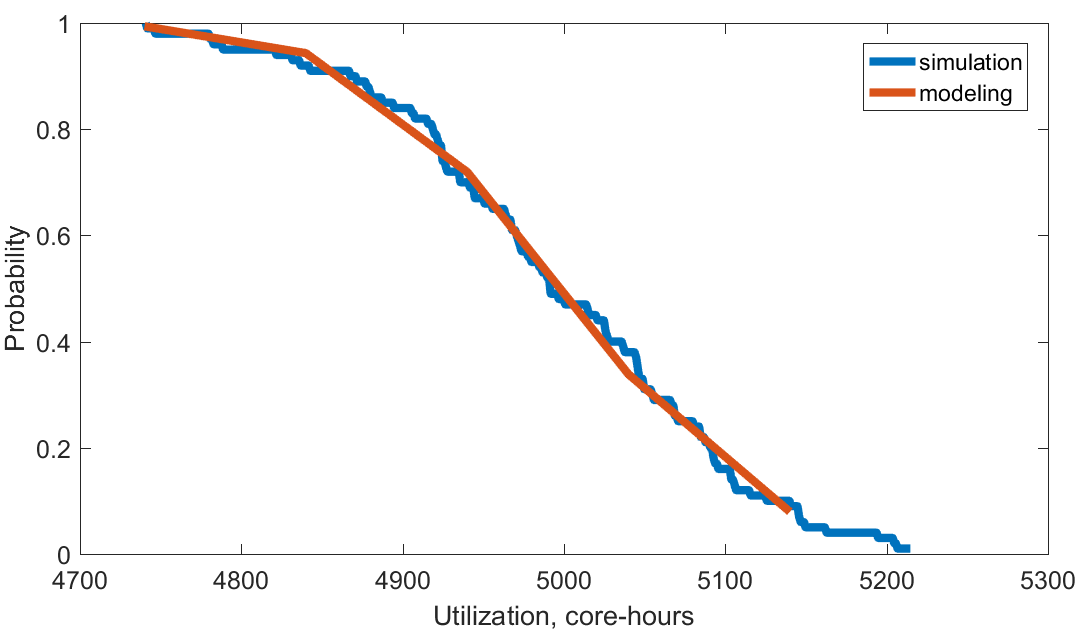
\includegraphics[width=0.48\textwidth]{pics/simulation-and-modeling.png}
    \caption{Probability (axis Y) that utilization will reach the corresponding utilization value (axis X) during the time of 5000 hours}
    \label{fig-simulation-and-modeling} 
\end{figure}
